\documentclass[1p]{elsarticle}        	% 5p gives 2 columns pr page, 1p gives 1.
\journal{Ingve Simonsen}
\usepackage{graphicx}
\usepackage{amsmath,amssymb}
\usepackage{booktabs}			% Nicer tables etc.
\usepackage{hyperref}
\usepackage[]{todonotes}

\usepackage{listings}
\usepackage{xcolor}
\lstset { %
    language=C++,
    backgroundcolor=\color{black!5}, % set backgroundcolor
    basicstyle=\footnotesize,% basic font setting
}

%\usepackage[section]{below}        %Confine figures to their sections

%%%%%%%%%%%%%%%%%%%%%%%%%%%%%%%%%%%%%%%%%%%%%%%%%%%%%%%%%%%%%%%%%%%%%%%%%
\begin{document}
\begin{frontmatter}
\title{Exam in TFY4235}
\author{Paul Thrane}
\begin{abstract}
This documents my work during the home exam in Computational Physics at NTNU. The task \cite{exam} considers a 1D reaction diffusion system, corresponding to the ones examined in \cite{einarsrud} and \cite{samseth}.
Accompanying this document should be a zip file containing the code I've written, together with the code and documentation for the the 2'nd assignment during the course \cite{percolation}.
During the exam I have discussed the problems with Kristian Hjorth, Rasmus Tran\aa s and H\aa kon Task\'en.

\end{abstract}
\end{frontmatter}
%%%%%%%%%%%%%%%%%%%%%%%%%%%%%%%%%%%%%%%%%%%%%%%%%%%%%%%%%%%%%%%%%%%%%%%%%
\section{Solving the Differential Equations}
I will not introduce the task, as this is explained in \cite{exam}, but for reference i have included the equations of interest;
\begin{subequations}
\begin{equation}
a_t = \partial_x (D_a \partial_xa) - Rab,
\end{equation}    
\begin{equation}
b_t = \partial_x (D_b \partial_xb) - Rab,
\end{equation}
\begin{equation}
c_t = \partial_x (D_c \partial_xc) + Rab - N_1\theta (c-c_0)c^2 - N_2cs,
\end{equation}
\begin{equation}
s_t = + N_1\theta (c-c_0)c^2 + N_2cs.
\end{equation}
\label{pde}
\end{subequations}

A major part of the first day went to examining these equations and understanding what they described. 
At first glance it seemed like it would be easy to implement an explicit scheme to solve them, but I did not know if this would converge nicely. 
I found several papers describing different angles of attack, for example \cite{kassam}, which states that a usual approach is low order finite differences but that higher order methods can be much faster. 
Nonetheless, I figured I would be better off implementing something i had done before. 
Having Assignment 3\footnote{Assignment 3 concerned low order Euler methods and related schemes.} fresh in mind, I decided I would test using an explicit scheme, as it then would be trivial to include the nonlinear cross terms in between the gasses and the solid.
 After a brief sidetrack trying to formulate a Lax-Wendroff scheme I further settled on using the lowest order since it would probably save time both in the implementation and for debugging. 
 Also, \cite{einarsrud} states that the reaction terms are fast, and that they therefore choose an explicit method. 
 This can be seen by writing the equations in a dimensionless form, where the reaction term will be multiplied by the factor $RL^2/D_g$, which for the relevant values of $R$, $L$ and $D$ is of the order of $10^7$.

I implemented the solution of the equations in C++, mainly because I figured speed might be an issue as well as it being my preferred language besides Python. 
I hesitated a bit when deciding how to structure the code. In the end, I decided on having everything in one file, since I did not think I would need that much code. 
Further, I decided to store the data in Armadillo vectors  \cite{armadillo}, and use their vector multiplication instead of using arrays and loops, mainly because I figured it would be more readable. 
The main loop that updates the solution to the next time step is the following:
\begin{lstlisting}
    // a + b -> c, NOTE: % is element wise multiplication in Armadillo
    reaction_ab = delta_t*R*(a%b);
    // Nucleation
    step_func(c, c0, above_critical_c);
    reaction_cc = delta_t*N1*(above_critical_c % (c%c));
    // Deposition on existing solids
    reaction_cs = delta_t*N2*(c%s);
    // Add reaction terms
    a = a - reaction_ab;
    b = b - reaction_ab;
    c = c + reaction_ab - reaction_cc - reaction_cs;
    s = s               + reaction_cc + reaction_cs;
    // Diffusion of gasses
    a = B_a*a;
    b = B_b*b;
    c = B_c*c;
\end{lstlisting}
Here, $B_a$, $B_b$ and $B_c$ are tridiagonal matrices giving diffusion of the gasses. Notice that the states are updated from the interaction separately from updating due to diffusion.
This was tested due to a comment in \cite{einarsrud} where it is stated that they do the same.
This can be considered reasonable since the reaction terms will be the same either way, while the produced gas $c$ should propagate with the diffusion coefficient $D_c$.
Also, it was found to be a little more stable to update due to the different effects separately.
Furthermore, this way of implementation opens up the possibility of using an implicit scheme for the diffusion terms.
The reason you would usually like to do this is to improve stability and thereby be able to take larger time steps without diverging from the correct solution.
Upon testing, it became clear that for the given values of the parameters the program diverged for larger time steps due to the diffusion term close to the border where b is large.
However, with an implicit solution I was still not able to increase the time step.
This was because the reaction term became unstable for approximately the same time step that the explicit scheme diverged, which can be understood by considering that the reaction term essentially works on a different timescale as stated above.
Because of this I decided to stick with the explicit solution, as it includes less calculations at the time resolution needed to handle the reaction terms.

In the above $D_g$ was assumed to be constant. For a spatially varying $D_g$ i decided to give up the matrix formulation of the diffusion term, since I found a nice way to update this using Armadillo's vector notation.
With 
\begin{equation}
\mathbf{D}_g = D_{g,0} \frac{1}{1+\mathbf{s}/s_0} = D_{g,0} \mathbf{u},
\end{equation}
I could write, using the notation that $u_\pm = u(t,x \pm \delta x)$,
\begin{equation}
g(t+\delta t, x) = g +  \frac{\delta t D_{g,0}}{4\delta x^2} (u_+ - u_-)( g_+ - g_-) + u \frac{\delta t D_{g,0}}{\delta x^2}(g_+ -2g + g_-).
\label{varyd}
\end{equation}
This resulted in the following procedure to update the states for a timestep, with diffusion\_varying\_D() applying \eqref{varyd}:
\begin{lstlisting}
    // a + b -> c, NOTE: % is element wise multiplication in Armadillo
    reaction_ab = delta_t*R*(a%b);
    // Nucleation
    step_func(c, c0, above_critical_c);
    reaction_cc = delta_t*N1*(above_critical_c % (c%c));
    // Deposition on existing solids
    reaction_cs = delta_t*N2*(c%s);
    // Add reaction terms
    a = a - reaction_ab;
    b = b - reaction_ab;
    c = c + reaction_ab - reaction_cc - reaction_cs;
    s = s               + reaction_cc + reaction_cs;
    // Diffusion of gasses
    // Varying D
    u = 1.0/(1.0+s/s0);
    diffusion_varying_D(delta_t, delta_x, N_grid, Da0, a, a, u);
    diffusion_varying_D(delta_t, delta_x, N_grid, Db0, b, b, u);
    diffusion_varying_D(delta_t, delta_x, N_grid, Dc0, c, c, u);
\end{lstlisting}

When looking at the reaction where 2 molecules of $a$ react with one of $b$, I have assumed that the reaction rate will be proportional to the square of concentration of  $a$ while being linear in that of $b$. Additionally, the reaction term must be subtracted twice from the concentration of $a$. This approach requires the reaction coefficient $R$ to be redefined, however this is expected since it describes another reaction.
\begin{lstlisting}
    // For 2a + b -> c, NOTE: % is element wise multiplication in Armadillo
    reaction_ab = delta_t*R*(a%a%b);
    // Nucleation
    step_func(c, c0, above_critical_c);
    reaction_cc = delta_t*N1*(above_critical_c % (c%c));
    // Deposition on existing solids
    reaction_cs = delta_t*N2*(c%s);
    // Add reaction terms
    a = a - 2*reaction_ab;
    b = b - reaction_ab;
    c = c + reaction_ab - reaction_cc - reaction_cs;
    s = s               + reaction_cc + reaction_cs;
    // Diffusion of gasses
    // Constant D
    a = B_a*a;
    b = B_b*b;
    c = B_c*c;
\end{lstlisting}

Since we get a lot of plots, I found it more tidy to describe the results and behavior of the system in corresponding figure captions.
The parameters used are listed in each figure. 
Additionally, a .mp4 file is included in the folder accompanying this document.
It shows the behavior of the system more dynamically than any of the static plots.

\begin{figure}
	\centering
	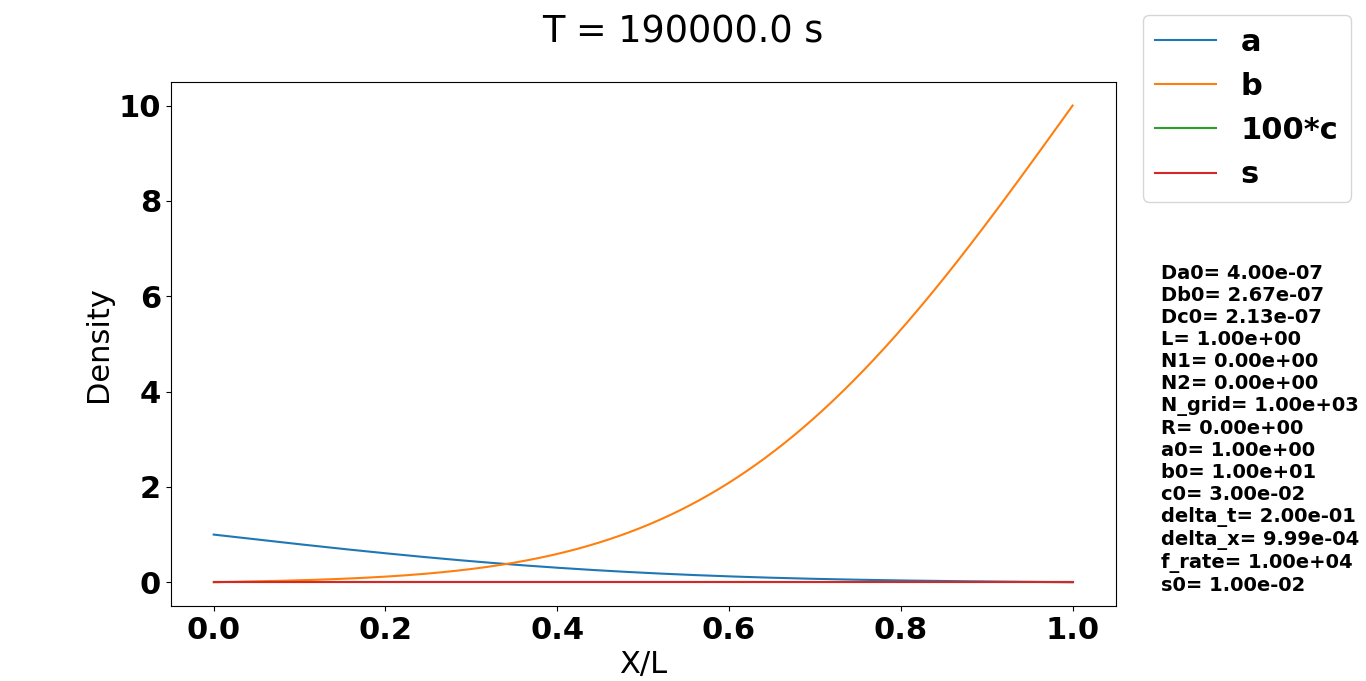
\includegraphics[width=\linewidth]{../figures/R0.png}
	\caption{Here $R$ is set to zero. I used this plot to check that my implementation of the diffusion term was correct. We get the expected form of diffusion for both $a$ and $b$. The used parameters are indicated. The f\_rate variable is used to indicate how often the loop should save output.}
	\label{fig:coords}
\end{figure}

\begin{figure}
	\centering
	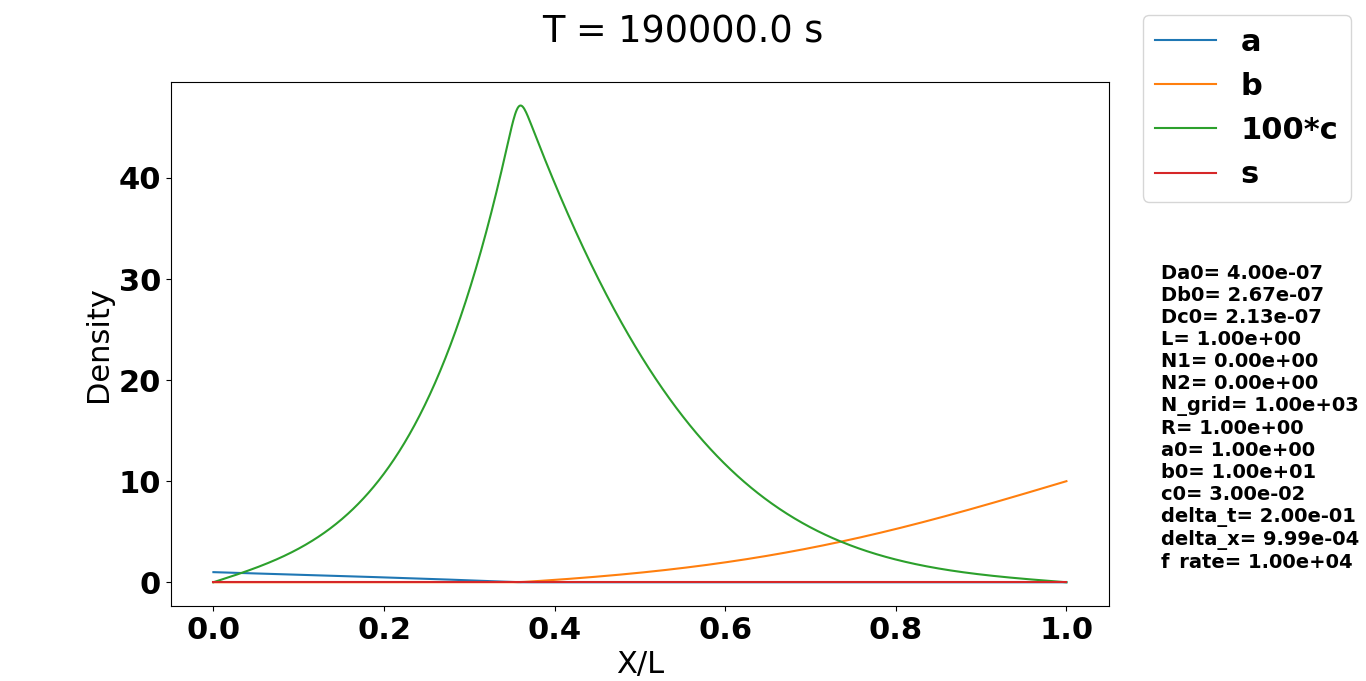
\includegraphics[width=\linewidth]{../figures/N0.png}
	\caption{Here $R$ is non-zero, but we have $N_1$ and $N_2$ zero, we see the production of $c$ as well as the diffusion of all thee gasses as expected.}
	\label{fig:coords}
\end{figure}

\begin{figure}[h]
	\centering
	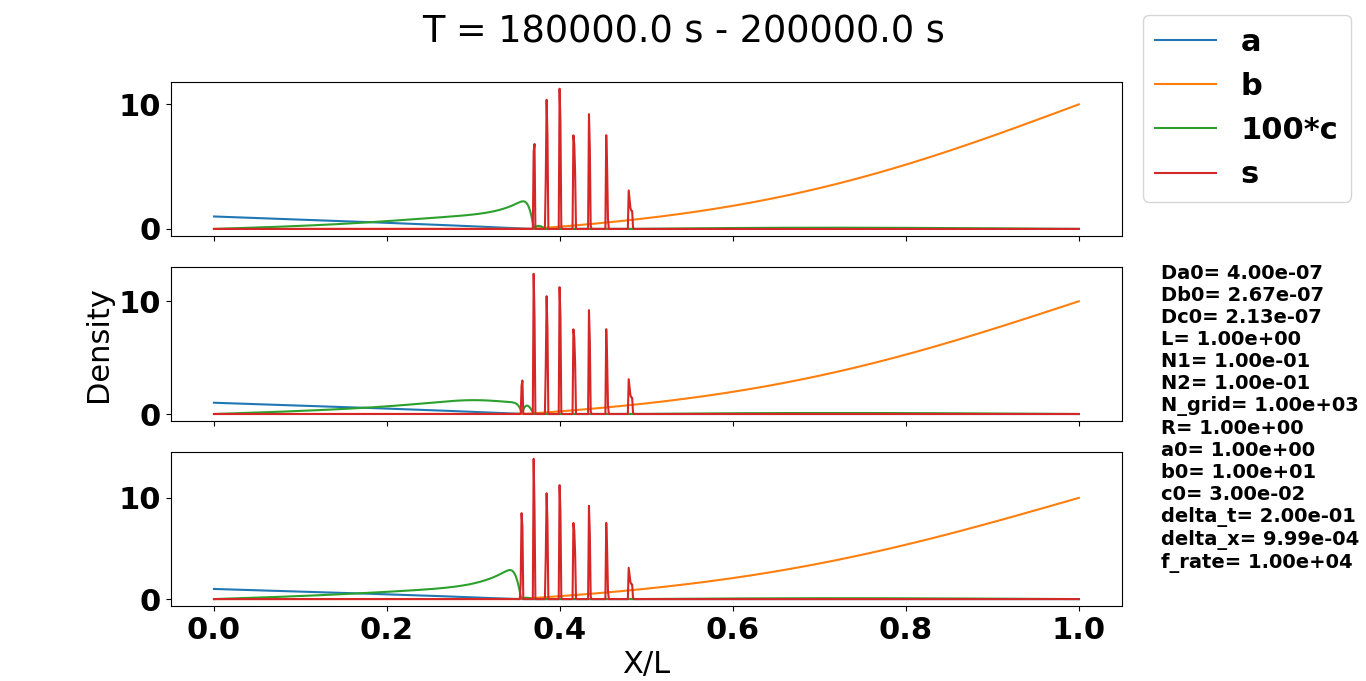
\includegraphics[width=\linewidth]{../figures/standard_settings_time.png}
	\caption{Here we have the standard values of the parameters as defined in the task, plotted for three different times to see the behavior. To see the time evolution better check the .mp4 file included in the accompanying folder. We see from the figure that $c$ has been produced until it reaches $c_0$ at some point, here shifted towards the left due to higher $b_0$. When we get a nucleation point for s and c is allowed to aggregate here, we get a peak that depletes the immediate surrounding for $c$. $b$ then propagates further to the left, making $c$ build up to $c_0$ again, but now shifted to the left. We see that the  remaining $c$ trapped between two peaks spreads, aggregating on the two nearest peaks.}
	\label{fig:coords}
\end{figure}

\begin{figure}
	\centering
	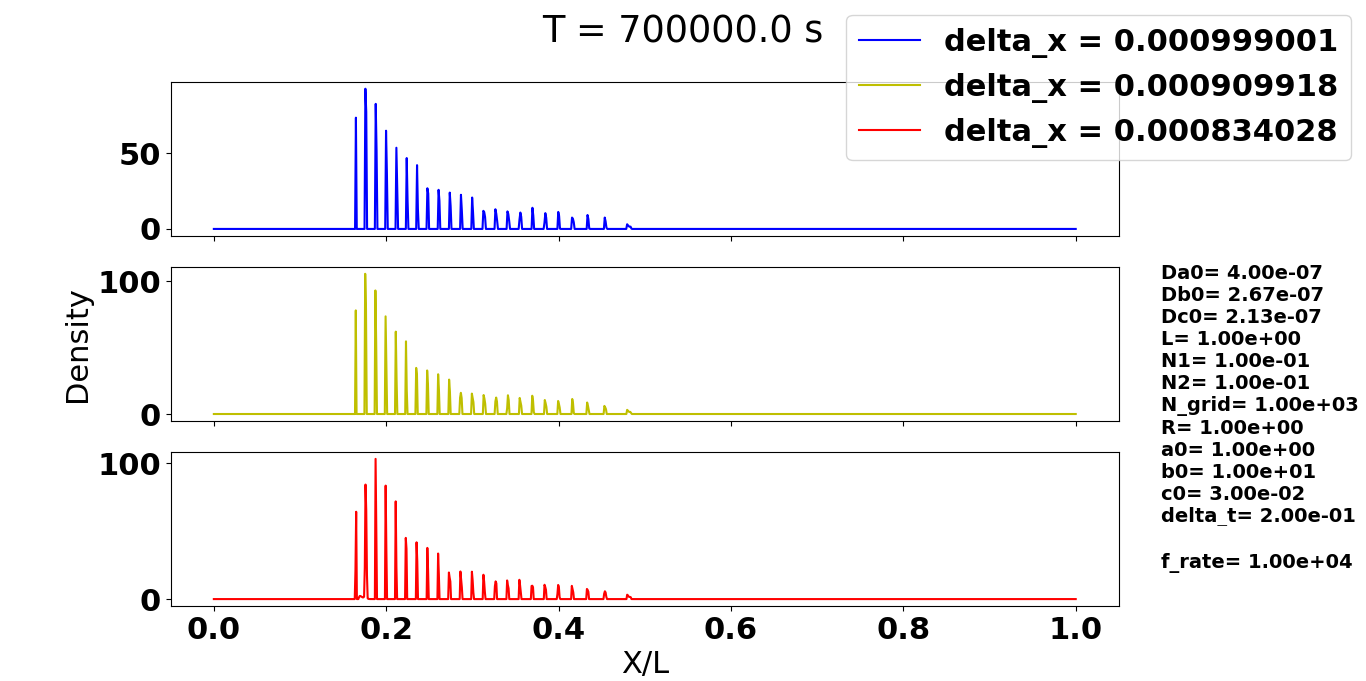
\includegraphics[width=\linewidth]{../figures/deltaX.png}
	\caption{Plot of standard choice of parameters but for three different step lengths in $x/L$. We see that there are some small variations in the peak heights, but these differences get smaller for smaller step lengths.}
	\label{fig:coords}
\end{figure}

\begin{figure}
	\centering
	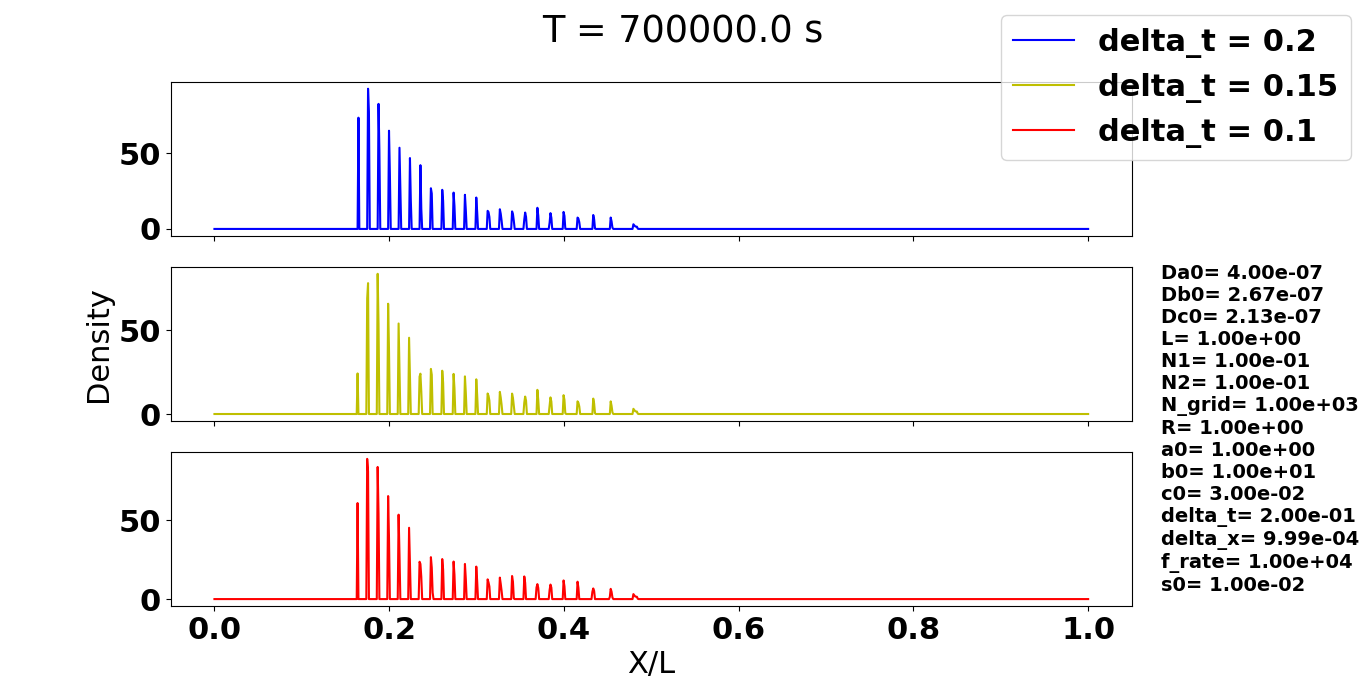
\includegraphics[width=\linewidth]{../figures/deltaT.png}
	\caption{Plot of standard choice of variables for different step lengths in time. Here the plots are almost identical. The differences for the final three peaks are due to small differences in the simulated total time resulting from different step lengths.}
	\label{fig:coords}
\end{figure}

\begin{figure}
	\centering
	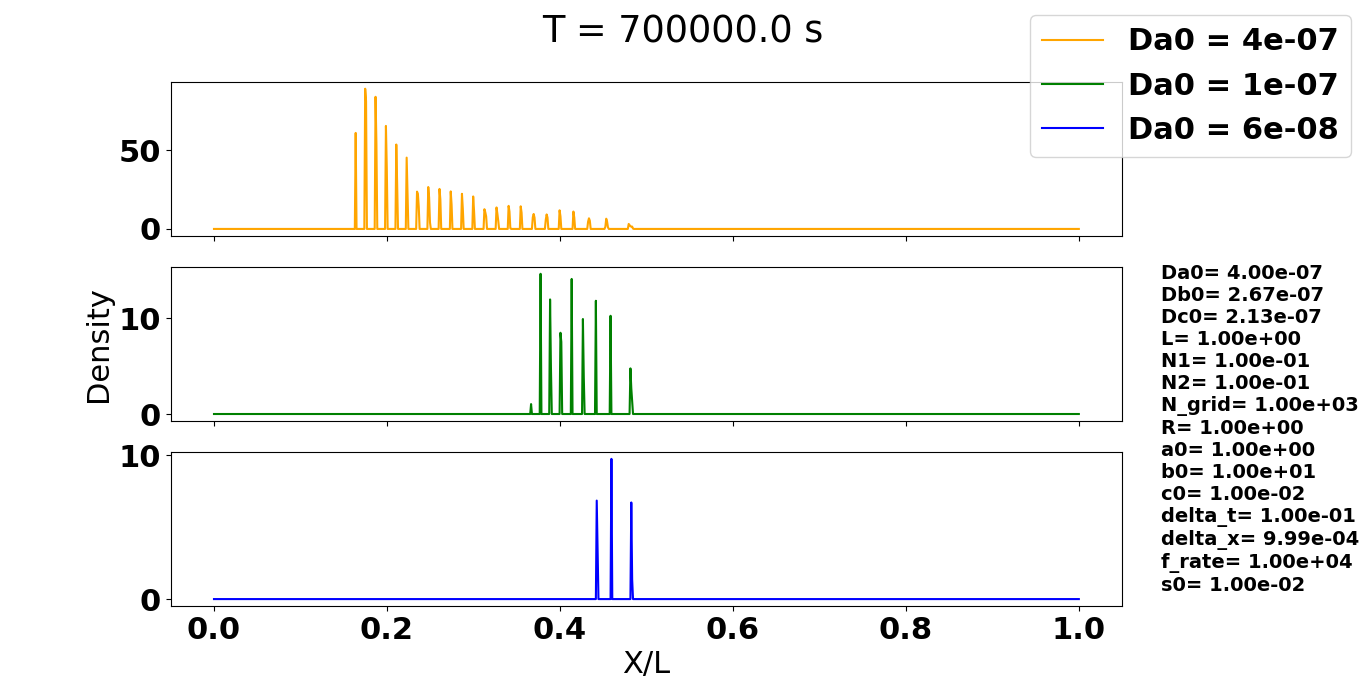
\includegraphics[width=\linewidth]{../figures/Da0_same_ratio.png}
	\caption{Coordinates.}
	\label{fig:coords}
\end{figure}

\begin{figure}
	\centering
	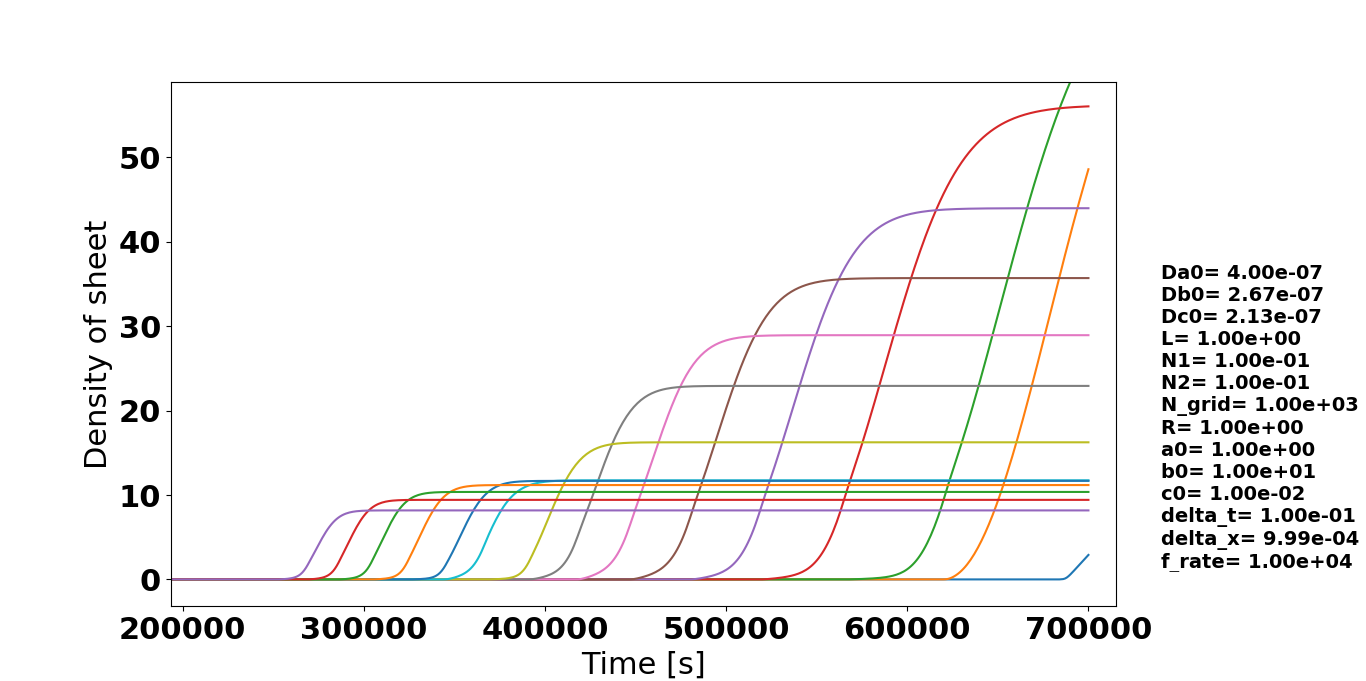
\includegraphics[width=\linewidth]{../figures/peak_growth.png}
	\caption{Coordinates.}
	\label{fig:coords}
\end{figure}

\begin{figure}
	\centering
	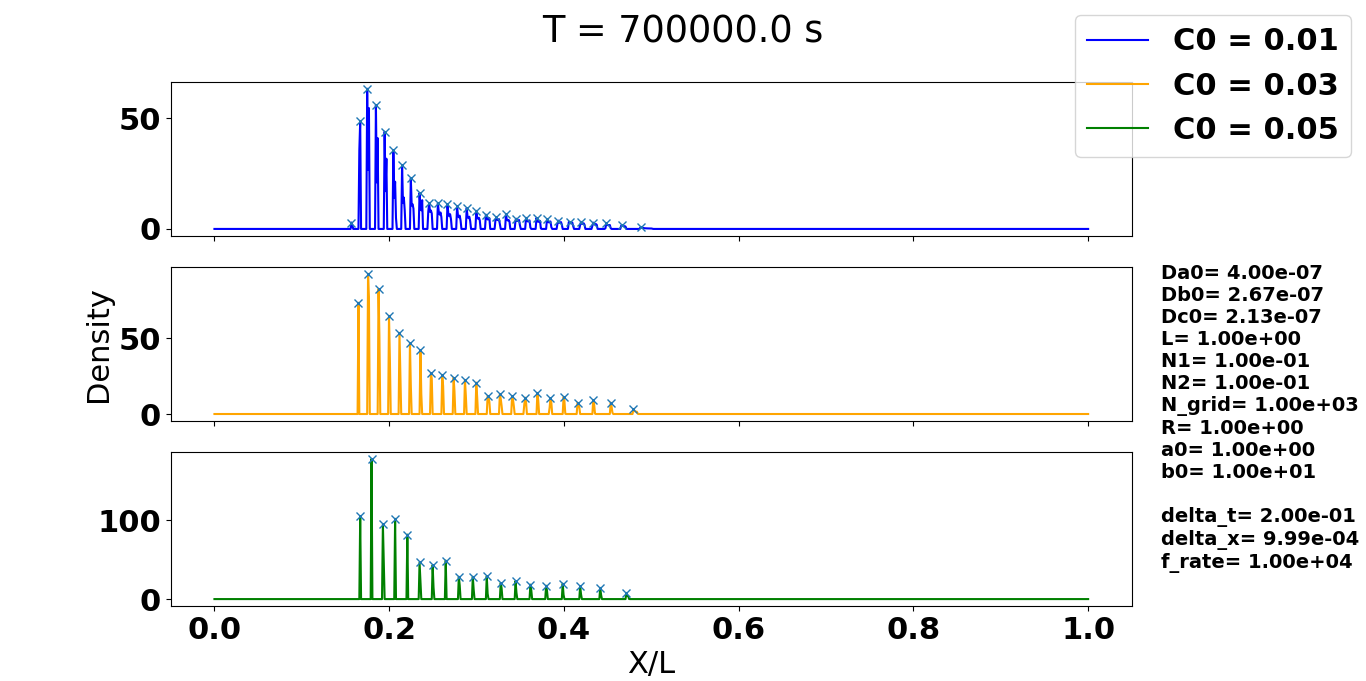
\includegraphics[width=\linewidth]{../figures/deltaC0_s.png}
	\caption{Coordinates.}
	\label{fig:coords}
\end{figure}

\begin{figure}
	\centering
	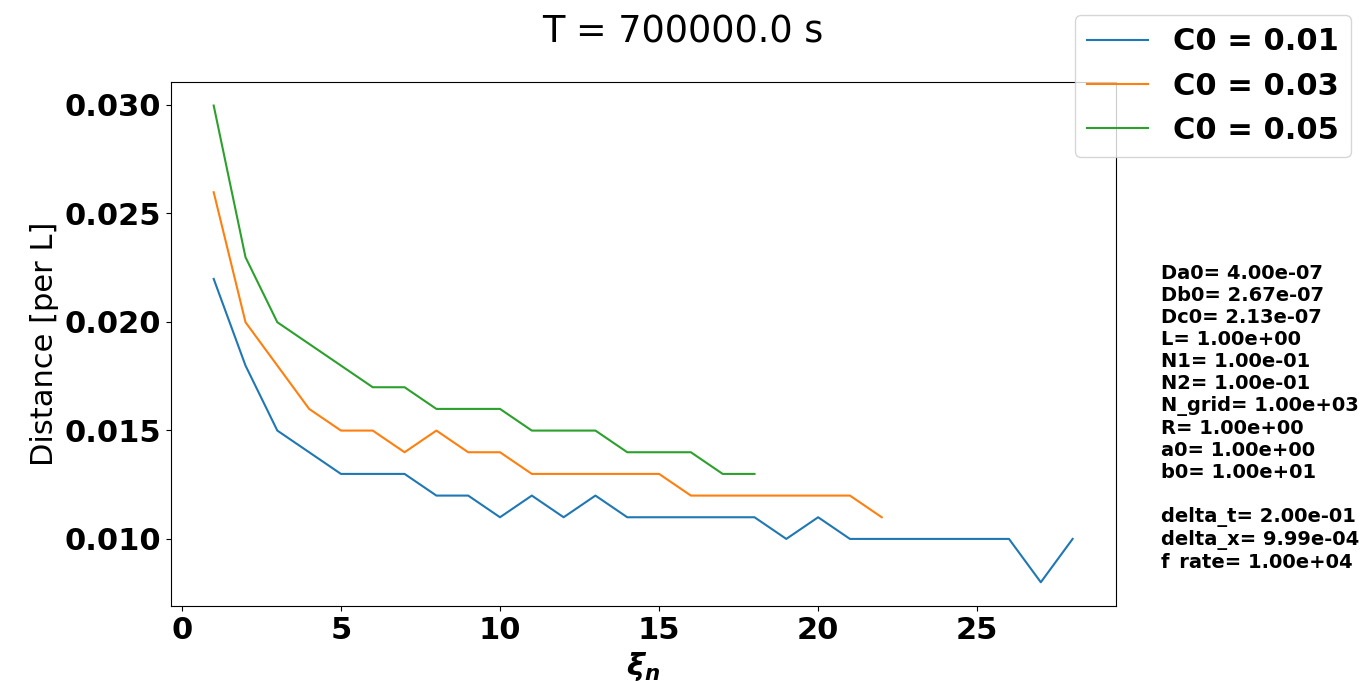
\includegraphics[width=\linewidth]{../figures/deltaC0_x.png}
	\caption{Coordinates.}
	\label{fig:coords}
\end{figure}

\begin{figure}
	\centering
	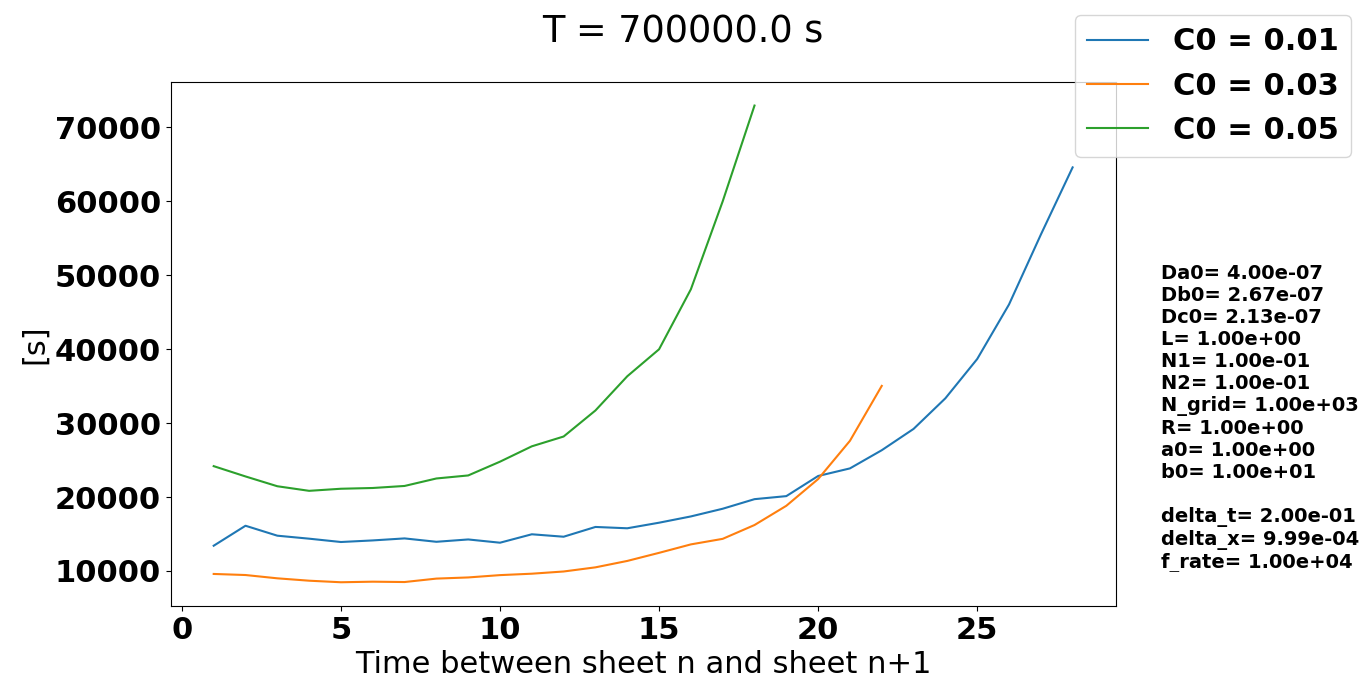
\includegraphics[width=\linewidth]{../figures/deltaC0_t.png}
	\caption{Coordinates.}
	\label{fig:coords}
\end{figure}

\begin{figure}
	\centering
	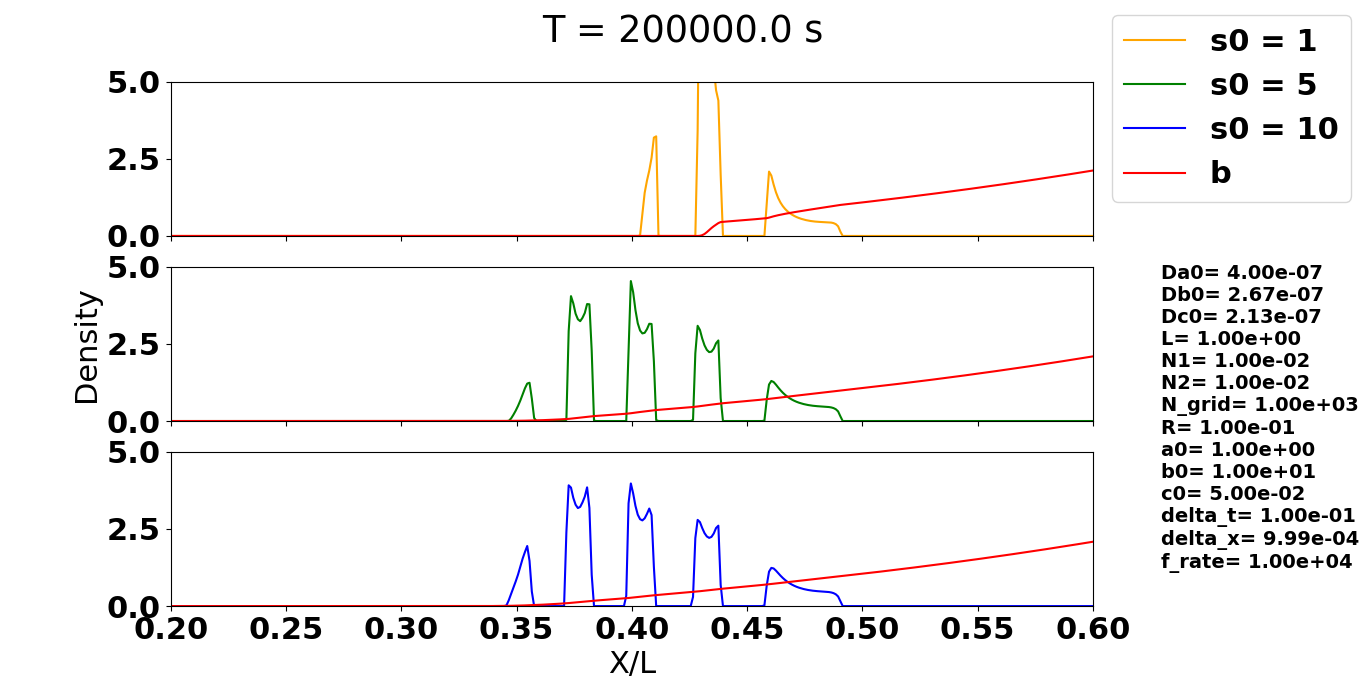
\includegraphics[width=\linewidth]{../figures/s0_1-10.png}
	\caption{Coordinates.}
	\label{fig:coords}
\end{figure}

\begin{figure}
	\centering
	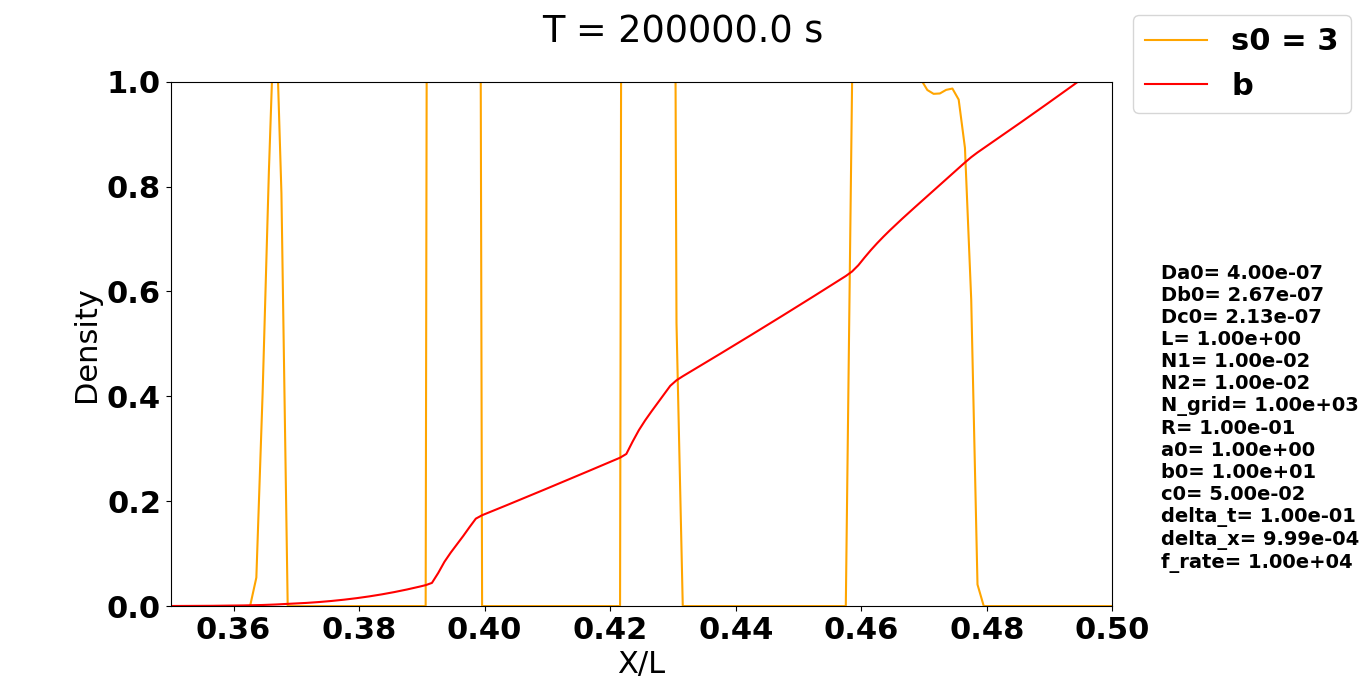
\includegraphics[width=\linewidth]{../figures/s0_3.png}
	\caption{Coordinates.}
	\label{fig:coords}
\end{figure}

\begin{figure}
	\centering
	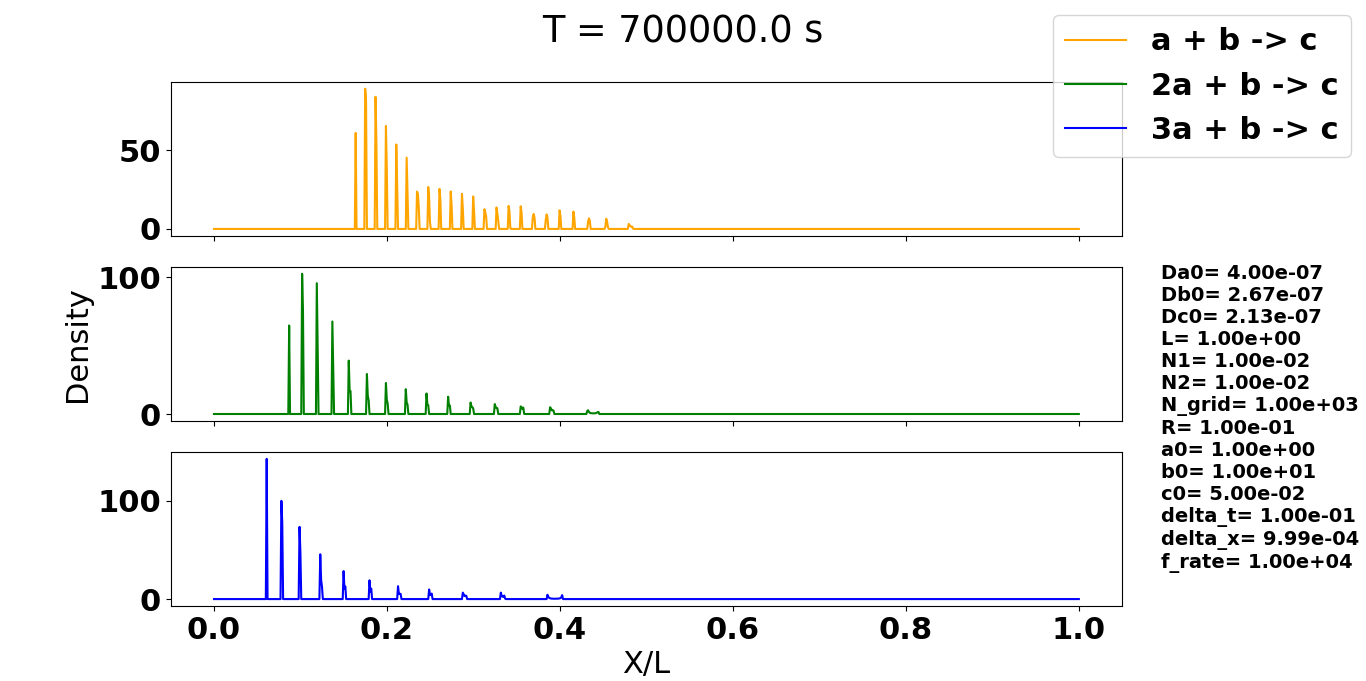
\includegraphics[width=\linewidth]{../figures/2a_s.png}
	\caption{Coordinates.}
	\label{fig:coords}
\end{figure}






\section*{References}
\bibliographystyle{elsart-num}
\bibliography{bibl}  

\end{document}